% !TEX root = scaling_book_exercises_replica.tex
\documentclass[10pt]{article}
\usepackage[a4paper,margin=17mm]{geometry}
\usepackage{amsmath,amssymb,array,booktabs}
\usepackage{tikz}
\usepackage{xcolor}
\usepackage{enumitem}
\usepackage{graphicx}
\usepackage{listings}
\usepackage[most]{tcolorbox}
\graphicspath{{./}{prism-uploads/}}
\setlength{\parindent}{0pt}
% Deliberately airy: the scanned original uses a generous notebook-line rhythm.
\setlength{\parskip}{0.9em}
\renewcommand{\arraystretch}{1.4}
\newcommand{\note}[1]{\textcolor{blue!55!black}{#1}}
\newcommand{\answer}[1]{\textcolor{blue!65!black}{\textbf{#1}}}
\newcommand{\question}[1]{\par\vspace{0.9em}\noindent\textbf{#1}\quad}
\newcommand{\meta}[2]{\textbf{#1} #2\hspace{2.5em}}
\newcommand{\allreduce}{\operatorname{AllReduce}}
\newcommand{\allgather}{\operatorname{AllGather}}
\newcommand{\rs}{\operatorname{ReduceScatter}}
\newcommand{\pagehead}[2]{%
 {\small\meta{DATE:}{#1}\meta{NO.:}{#2}\meta{SUBJECT:}{Scaling Book Exercises}}\par\vspace{0.8em}\hrule\vspace{0.8em}}
\lstdefinestyle{pythonstyle}{
  language=Python,
  basicstyle=\ttfamily\small,
  breaklines=true,
  showstringspaces=false,
  columns=fullflexible,
  numbers=left,
  numberstyle=\tiny\color{gray!70},
  numbersep=8pt,
  keywordstyle=\color{blue!60!black}\bfseries,
  stringstyle=\color{red!65!black},
  commentstyle=\color{teal!65!black}\itshape
}
\lstdefinestyle{terminal}{
  language={},
  basicstyle=\ttfamily\small,
  breaklines=true,
  showstringspaces=false,
  columns=fullflexible,
  numbers=left,
  numberstyle=\tiny\color{gray!70},
  numbersep=8pt,
  literate={±}{{$\pm$}}1 {µ}{{$\mu$}}1
}
\newtcblisting{pythonblock}[1]{
  enhanced,
  breakable,
  listing only,
  listing engine=listings,
  listing options={style=pythonstyle},
  colback=white,
  colframe=green!35!gray,
  boxrule=0.8pt,
  sharp corners,
  left=5pt,
  right=5pt,
  top=7pt,
  bottom=5pt,
  title={Python Code: #1},
  fonttitle=\bfseries,
  coltitle=black,
  colbacktitle=green!18,
  attach boxed title to top left={xshift=7mm,yshift*=-\tcboxedtitleheight/2},
  boxed title style={sharp corners,boxrule=0pt,colframe=green!18}
}
\newtcblisting{compactpythonblock}[2][]{
  enhanced,
  listing only,
  listing engine=listings,
  listing options={style=pythonstyle,basicstyle=\ttfamily\scriptsize},
  colback=white,
  colframe=green!35!gray,
  boxrule=0.8pt,
  sharp corners,
  left=4pt,
  right=4pt,
  top=5pt,
  bottom=3pt,
  title={Python Code: #2},
  fonttitle=\bfseries,
  coltitle=black,
  colbacktitle=green!18,
  attach boxed title to top left={xshift=7mm,yshift*=-\tcboxedtitleheight/2},
  boxed title style={sharp corners,boxrule=0pt,colframe=green!18},
  #1
}
\newtcblisting{terminalblock}[2][]{
  enhanced,
  breakable,
  listing only,
  listing engine=listings,
  listing options={style=terminal},
  colback=white,
  colframe=blue!30,
  boxrule=0.8pt,
  sharp corners,
  left=5pt,
  right=5pt,
  top=7pt,
  bottom=5pt,
  title={Terminal Output: #2},
  fonttitle=\bfseries,
  coltitle=black,
  colbacktitle=blue!12,
  attach boxed title to top left={xshift=7mm,yshift*=-\tcboxedtitleheight/2},
  boxed title style={sharp corners,boxrule=0pt,colframe=blue!12},
  #1
}
\begin{document}
\linespread{1.16}\selectfont
\raggedbottom
\begin{titlepage}
  \centering
  \vspace*{0.30\textheight}
  {\LARGE Scaling Law Report\par}
  \vspace{1.2em}
  {\large Kanson Chu\par}
  \vspace{0.6em}
  {\large August 8, 2026\par}
  \vfill
\end{titlepage}

\begin{titlepage}
  \centering
  {\LARGE\textbf{Contents}\par}
  \vspace{2em}
  \begin{minipage}{0.45\textwidth}
  \begin{enumerate}[leftmargin=2em]
    \item Notes
    \item Exercises Writeups
      \begin{itemize}[leftmargin=2em]
        \item Section 1
        \item Section 2
        \item Section 3
      \end{itemize}
  \end{enumerate}
  \end{minipage}
  \vfill
\end{titlepage}
\setcounter{page}{3}


\begingroup
\setlength{\parskip}{0pt}
\centering
{\small\textit{Original handwritten notes from the reverse of my notebook cover,\linebreak
collecting key ideas and working sketches from my reading.}\par}
\vspace{0.8em}
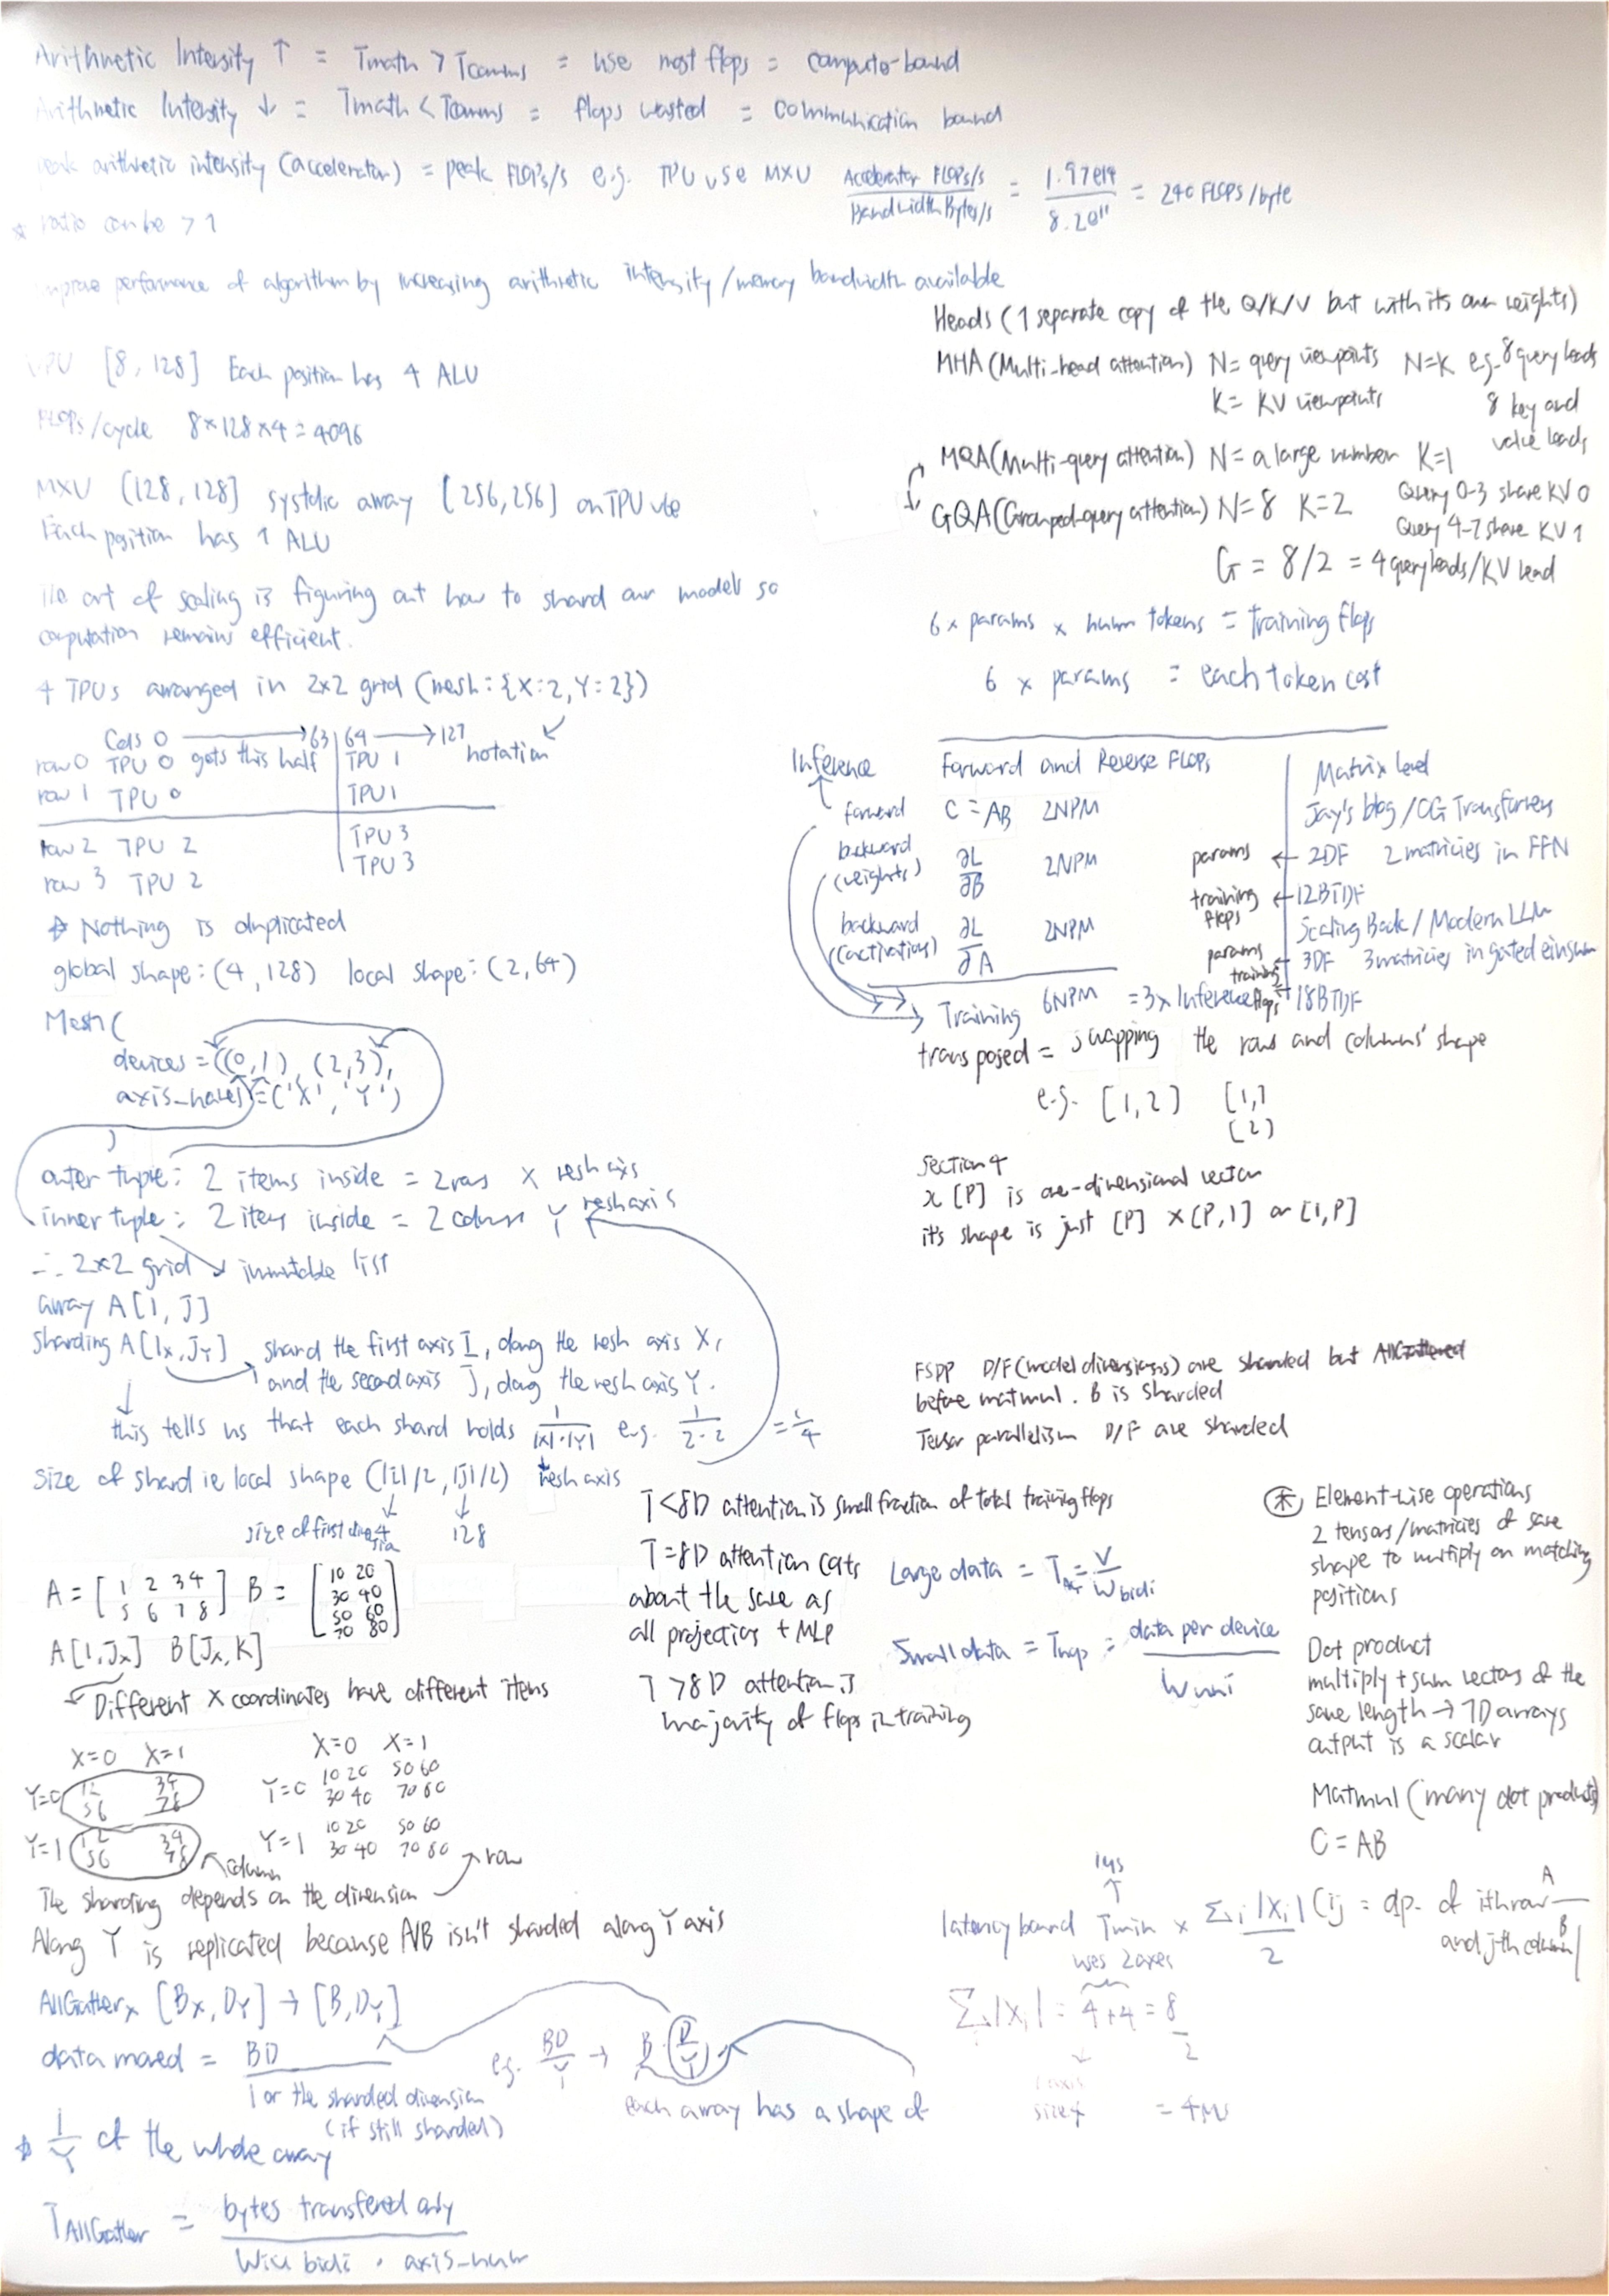
\includegraphics[page=1,width=\textwidth,height=0.86\textheight,keepaspectratio]{Cover Notes.pdf}\par
\endgroup
\clearpage

\pagehead{13 / 7 / 2026}{Section 1}
\question{Q1.1.}$X[B,D]$, $Y[D,F]$\hfill \answer{Need to load from memory: $BD+DF$}\\
\hfill \answer{Need to be written back to memory: $BF$}

\begin{enumerate}[label=\arabic*.,leftmargin=1.4em,start=2]
\item dot product: $D + D - 1 = 2D - 1 \approx 2D$ \hfill \answer{Total OPs: $2BDF$}\\
$[B,F]$: output grid of numbers. \quad Total OPs: $2BDF$.
\item $\dfrac{2BDF}{BD+DF+BF}=\dfrac{\text{Total OPs}}{\text{Total Comms}}$.
\end{enumerate}
\answer{Arithmetic intensity (for algo): $\dfrac{2BDF}{BD+DF+BF}\approx\textcolor{black}{\dfrac{2BDF}{DF}=2B}$.}\\
\answer{Arithmetic intensity (for accelerator): $\dfrac{3.94\times10^{14}}{8.2\times10^{11}}=480$; \textcolor{black}{$2B>480$, $B>240$}.}

\begin{enumerate}[label=\arabic*.,leftmargin=1.4em,start=4]
\item $T_{\rm math}=\dfrac{\text{FLOPs}}{\text{Accelerator FLOPs/s}}$, \quad $T_{\rm comms}=\dfrac{\text{bytes}}{\text{bandwidth (bytes/s)}}$.\\
\answer{Upper bound: $T_{\rm math}+T_{\rm comms}$.}\\
\answer{Lower bound: $\max(T_{\rm math},T_{\rm comms})$.}\\
$T_{\rm math}=\dfrac{2BDF}{3.94\times10^{14}}$, \quad $T_{\rm comms}=\dfrac{BD+DF+BF}{8.2\times10^{11}}$.
\end{enumerate}

\question{Q2.}$2B>480$; \answer{Batch size: $B>240$.}\\
Arithmetic intensity (for algo): $\dfrac{2BDF}{2BD+DF+2BF}=\dfrac{2BDF}{DF}=2B$, hence $2B>240$, $B>120$.

\begin{center}\fbox{$\texttt{bf16[B,D]}\;*\;\texttt{int8[D,F]}\longrightarrow\texttt{bf16[B,F]}$}\end{center}
\small Input activations $\rightarrow$ batch size; static $\rightarrow$ output dimension; weights; compute.\normalsize

\newpage
\pagehead{13 / 7 / 2026}{Section 1}
\question{Q3.}$y$-axis: peak FLOPs/s; $x$-axis: batch size; \quad \texttt{numpy}: average $(1,500)$.\\
Total flops $=2BDF$, \quad $T_{\mathrm{math}}=\dfrac{2BDF}{1.97\times10^{14}}$,\\
$T_{\mathrm{comms}}=\dfrac{2BD+DF+2BF}{8.2\times10^{11}}$.\\
total time $=\max(T_{\mathrm{math}},T_{\mathrm{comms}})$; peak FLOPs/s $=\dfrac{2BDF}{\text{total time}}$.

\vspace{1em}
\begin{pythonblock}{Roofline Plot}
import matplotlib.pyplot as plt
import numpy as np

batch_size = np.arange(1, 500)

def peak_flops_per_second(B, D, F):
    total_flops = 2 * B * D * F
    t_math = total_flops / 1.97e14
    t_comms = (2 * B * D + D * F + 2 * B * F) / 8.2e11
    total_time = np.maximum(t_math, t_comms)
    return total_flops / total_time

roofline_4096 = peak_flops_per_second(batch_size, 4096, 4096)
roofline_1024 = peak_flops_per_second(batch_size, 1024, 1024)

plt.plot(batch_size, roofline_4096, label='D=F=4096')
plt.plot(batch_size, roofline_1024, label='D=F=1024')
plt.xlabel('Batch Size')
plt.ylabel('Peak FLOPs/s')
plt.legend()
plt.grid()
\end{pythonblock}

\begin{center}
  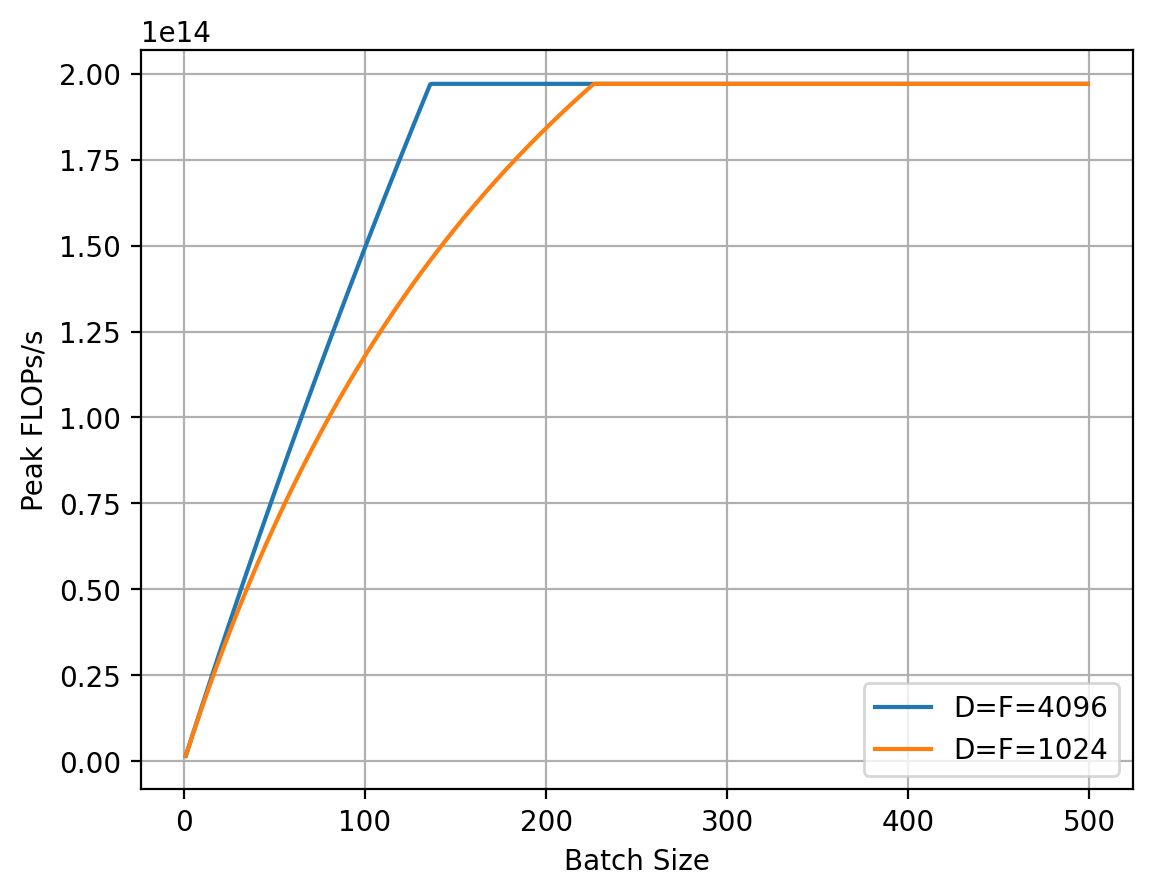
\includegraphics[width=0.65\textwidth]{Roofline Graph.png}\\*[-0.2em]
  {\small\textit{Peak FLOPs/s as a function of batch size for two matrix dimensions.}}
\end{center}

\question{Q4.}Arithmetic intensity $=\dfrac{\text{total ops}}{\text{total bytes}}$.\\
total ops: $D+D-1\approx2D$ (dot product); $[1,D]\cdot[D,F]=[1,F]$; $2DF\times B=2BDF$.\\
total bytes: $BD+BDF+BF$.\hfill \answer{Arithmetic intensity: $\dfrac{2BDF}{BD+BDF+BF}=\dfrac{2BDF}{BDF}=2$.}

\question{Q5.}Arithmetic intensity (H100 SXM): $\dfrac{1979\times10^{12}\div 2}{3.35\times10^{12}}=295$ FLOPs/byte.\\
$[B,D],D[D,F]\rightarrow[B,F]$; total OPs $=2BDF$; total comm $=2BD+2DF+2BF$; $\dfrac{2BDF}{2DF}=B$.\\
\answer{$B_{\rm crit}\ge 295$.}

\newpage
\pagehead{16 / 7 / 2026}{Section 2}
\question{Pop Quiz Appendix A.}\\
$8\times128\times4=4096$ FLOPs/cycle; $1.75\times10^9$ cycle/s; $4096\times1.75\times10^9=$ \textcolor{blue!65!black}{$7.168\times10^{12}$ FLOPs/s}.\\
Calculate FLOPs/cycle first then times cycle/s.

\question{Q1.}$200\mathrm{B}=200\times10^9$; $200\times10^9\times2=400\times10^9$ B; $400\times10^9\div32=1.25\times10^{10}$; $1.25\times10^{10}/1.2\times10^{12}=10.4$ ms. \hfill \answer{10.4 ms}

\question{Q2.}
\begin{tabular}[t]{@{}ll@{\qquad}ll@{}}
TPU v5e pod & & TPU v5p pod &\\
Hosts: & \answer{32} & Hosts: & \answer{2240}\\
Tensor Cores: & \answer{256} & Tensor Cores: & \answer{17920}\\
Total FLOPs/s (whole pod): & $5.0432\times10^{16}$ & Total FLOPs/s (whole pod): & $4.11264\times10^{18}$\\
Total HBM: & \answer{4096 GB} & Total HBM: & \answer{860160 GB}
\end{tabular}

\question{Q3.}$T_{\mathrm{math}}>T_{\mathrm{comms}}$: compute bound.\\
$\dfrac{2BDF}{9.2\times10^{14}}>\dfrac{2(BD+DF+BF)}{1.6\times10^{10}}$.\\
With $F=4D$,
\[
\dfrac{2BD(4D)}{9.2\times10^{14}}>\dfrac{2\bigl(BD+4D(D)+B(4D)\bigr)}{1.6\times10^{10}}.
\]
Neglecting the activation terms $BD$ and $B(4D)$ relative to $4D^2$,
\[
\dfrac{8BD^2}{9.2\times10^{14}}>\dfrac{8D^2}{1.6\times10^{10}}
\quad\Longrightarrow\quad B>\dfrac{9.2\times10^{14}}{1.6\times10^{10}}=57{,}500.
\]
\answer{$B>57{,}500$.}\hfill Use prior knowledge sometimes.

\newpage
\pagehead{17 / 7 / 2026}{Section 2}
\question{Q4.(1)}$T_{\rm math}=\dfrac{2B(4096)(16384)}{3.94\times10^{14}}=3.4\times10^{-7}B$.\\
$T_{\rm comms}=\dfrac{B(4096)+4096(16384)+B(16384)}{8.2\times10^{11}}$.\\
$\max(T_{\rm math},T_{\rm comms})=\left(3.4\times10^{-7}B,\dfrac{B(4096)+4096(16384)+B(16384)}{8.2\times10^{11}}\right)$.\\
$3.4\times10^{-7}B>\dfrac{4096B+4096(16384)+B(16384)}{8.2\times10^{11}}$; \answer{$B>267$.}

\textbf{(2)}\quad $\mathrm{VMEM}=\mathrm{HBM\ BW}\times22=8.2\times10^{11}\times22=1.804\times10^{13}$.\\
\answer{$B>11$.} \quad \note{around 20 in practice if loaded from VMEM.}

\newpage
\pagehead{18 / 7 / 2026}{Section 2}
\question{Q5.(1)}
$\begin{bmatrix}0,0&0,1&0,2&0,3\\1,0&1,1&1,2&1,3\\2,0&2,1&2,2&2,3\\3,0&3,1&3,2&3,3\end{bmatrix}$\quad
$\dfrac{2\times8\times128\times8192}{2\times4.5\times10^{10}}=186\,\mu s$.\\
$6\times1=6\,\mu s$; \answer{$6\,\mu s$ for first byte.}\\
\textbf{Q5.(2)}\quad \answer{$186+6=192\,\mu s$ total time.}

\question{Q6.}PCIe to TPUs respectively mapping: $(128\times1024)^2\div(16\times1.6\times10^{10})$; each TPU has $1.07$ GB.\\
$178$ ms $\rightarrow$ TPU $(0,0)$; all TPUs; load bf16 $[8,128,1024]$ ($2$ MB); $2.5\times10^{-3}$ s.\\
load HBM matrix to MXU: $20$ ms; total $1.4$ ms; \answer{upper bound $266.4$ ms}; \answer{lower bound $178$ ms}; \answer{real case $\approx200$ ms.}

\newpage
\pagehead{21 / 7 / 2026}{Section 3}
\question{Pop Quiz 1 [2D sharding across 1 axis].}\\
$\left[\dfrac{1024}{8\times2},\,4096\right]=[64,4096]$ per device.\\
$64\times4096\times4=1{,}048{,}576$ B.\\
\answer{Data per device (bytes): $1{,}048{,}576$ B.}\quad \answer{Time to load from HBM: $3.08\times10^{-7}$ s.}

\question{Pop Quiz.}$\left[\dfrac{128}{2\times8},\,2048\right]=[8,2048]$ per device.\\
$128\times2048\times2=524288$ B.\\
per device memory: $16384$ B; total memory $=524288$ B.\\
\note{Just make sure to shard the array in every mesh axis, or else the original array will have $k$ replicas, where $k$ is the number of axes you did not shard. This is also known as partially-replicated.}\\
\note{Shard all mesh axes $(x,y,z)$ to ensure no duplication in any place.}

\question{Pop Quiz 2 [AllGather time].}\\
Total $T_{\rm total}=\dfrac{2\times2048\times8192}{9\times10^{10}}\approx373\,\mu s>3\,\mu s$ (latency bound), so not latency-bound.\\
Unidirectional $T_{\rm total}=\dfrac{3\times8{,}388{,}608}{4.5\times10^{10}}\approx559\,\mu s$.\\
Part 2: $T_{\rm hop}=\dfrac{(256/4)\cdot256\cdot2}{4.5\times10^{10}}\approx0.7\,\mu s<1\,\mu s$; total $=\max(\text{latency},\text{bandwidth time})$, $3\cdot1\,\mu s=3\,\mu s$.\\
\answer{ideal total $=373\,\mu s$; unidirectional total $=559\,\mu s$; $T_{\rm hop}\approx0.7\,\mu s<1\,\mu s$, total $=3\,\mu s$.}

\newpage
\pagehead{24 / 7 / 2026}{Section 3}
\question{Q1.}$\dfrac{Y\cdot Z\cdot\mathrm{size\ of\ }A}{\mathrm{size\ }A}=\dfrac{8\cdot2}{1}=16$; \answer{16:1.}

\question{Q2.}Two equivalent layouts of a $4\times4$ matrix:
\[
\begin{array}{c@{\qquad}c}
\begin{bmatrix}1&2&3&4\\5&6&7&8\\9&10&11&12\\13&14&15&16\end{bmatrix}&
\begin{bmatrix}1&2&3&4\\5&6&7&8\\9&10&11&12\\13&14&15&16\end{bmatrix}
\end{array}
\]
Mesh axes: $x_0,x_1,x_2,x_3$ and $y_0,y_1,y_2,y_3$; $Y_{\rm out}=Y_{\rm inp}$.\\
\note{If we use the idling $z$ axis, parts 1 and 2 become shorter, e.g. $\dfrac{2BD}{2YW}=11.6\,\mu s$ (almost twice faster).}
\[
\begin{array}{lll}
\text{Pt 1:}&\dfrac{2BD}{YW}=\dfrac{2(1024)(4096)}{4(9\times10^{10})}\approx23\,\mu s,&\text{latency: }\dfrac{4}{2}=2\,\mu s\\[0.6em]
\text{Pt 2:}&\dfrac{2BD}{ZW}=\dfrac{2(1024)(4096)}{2(9\times10^{10})}\approx46\,\mu s,&\text{latency: }\dfrac{4+4}{2}=4\,\mu s\\[0.6em]
\text{Pt 3:}&2\cdot\dfrac{2BD}{XYW}=\dfrac{4BD}{XYW}=\dfrac{4(1024)(4096)}{(4)(4)(9\times10^{10})}\approx11\,\mu s,&\text{latency: }\dfrac{4}{2}=2\,\mu s\\[0.6em]
\textcolor{blue!65!black}{\text{Pt 2 }\mathrm{AG}_{XYZ}:}&\textcolor{blue!65!black}{\dfrac{2BD}{3W}=31\,\mu s.}&
\end{array}
\]
\note{Real-World Practice times.}

\newpage
\pagehead{26 / 7 / 2026}{Section 3}
\question{Q3.}$\dfrac{4}{2}\times1\,\mu s=2\,\mu s$; $\dfrac{2(128)}{4}=64$ B/device.\\
$T_{\rm hop}=\dfrac{64}{4.5\times10^{10}}\approx1.42\times10^{-9}$ s, negligible compared with $1\,\mu s$.\\
\answer{$2\,\mu s$; $1\,\mu s$ per hop latency; $2\,\mu s$ overall latency bound.}

\question{Q4. Strategy 1}$T_{\rm total}=\max\left(\dfrac{2BDF}{C},\dfrac{2DF}{Wici}\right)$.\\
$\dfrac{2DF}{Wici}>\dfrac{2BDF}{C}$; $\dfrac{C}{Wici}>B$; \answer{$B<2550$} (comms bound).\\
$T_{\rm comms,2}<T_{\rm comms,1}$:
\[
\dfrac{4BF}{Wici}<\dfrac{2DF}{Wici}
\quad\Longrightarrow\quad 2B<D.
\]
\answer{$D>2B$.}\quad Usually true because $D$ is large and $B$ is small.\\
$T_{\rm comms,2}<T_{\rm math,1}$:
\[
\dfrac{4BF}{Wici}<\dfrac{2BDF}{C}
\quad\Longrightarrow\quad \dfrac{C}{Wici}<\dfrac{D}{2}
\quad\Longrightarrow\quad D>5100.
\]
\answer{$D>5100$.}

\question{Strategy 2}$T_{\rm total}=\max\left(\dfrac{2BDF}{XC},\dfrac{4BF}{Wici}\right)$.\\
Comms bound when
\[
\dfrac{4BF}{Wici}>\dfrac{2BDF}{XC}
\quad\Longrightarrow\quad \dfrac{2}{Wici}>\dfrac{D}{XC}
\quad\Longrightarrow\quad \dfrac{C}{Wici}>\dfrac{D}{2X}.
\]
$5100>D/X$, so $X>D/5100$; \answer{$X<1.56\approx2$.}\\
\note{Always comms bound almost.}

\begin{center}\answer{Strategy 2 is better than Strategy 1}\end{center}
\begin{center}\begin{tabular}{llll}\toprule
Batch size $B$ & Strategy 1 bound type & Strategy 2 faster if & Usually true?\\\midrule
$B<2550$ & comms bound & $D>2B$ & Yes\\
$B>2550$ & compute bound & $D>5100$ & Yes (large models)\\\bottomrule
\end{tabular}\end{center}

\newpage
\pagehead{27 / 7 / 2026}{Section 3}
\question{Q5.}$A[I,J_{XYZ}]\cdot B[J_{XYZ},K]\to\allreduce_{XYZ}(C[I,K]\{U_{XYZ}\})$.\\
Compute time $=\dfrac{2IJK}{XYZC}$; communication time $=\dfrac{4IK}{Wici}$.\\
Alternatively, shard a non-contracting dimension:
\[
A[I_{XYZ},J]\cdot B[J,K]\to\allgather_{XYZ}(C[I_{XYZ},K])
\]
or
\[
\boxed{A[I,J]\cdot B[J,K_{XYZ}]\to\allgather_{XYZ}(C[I,K_{XYZ}])}
\]
Compute time $=\dfrac{2IJK}{XYZC}$; communication time $=\dfrac{2IK}{Wici}$.\\
\note{Sharded over all three mesh axes $X,Y,Z$, hence per-device FLOPs are $1/(XYZ)$ of the unsharded FLOPs. Here $XYZ$ in the denominator denotes the product of the mesh-axis sizes. Both AllGather alternatives produce the replicated output $C[I,K]$.}

\question{Q6.}Time pairs below are $(T_{\rm math},T_{\rm comms})$.\\
\begin{tabular}{@{}ll@{\qquad}ll@{}}
P1: & $A[I_X,J_Y]\cdot B[J_Y,K]\to C[I_X,K]$, & comm primitive: & $\allreduce_Y(C[I_X,K]\{U_Y\})$\\
 & $\left(\dfrac{2IJK}{XYC},\dfrac{4IK}{XWici}\right)$ && \\[0.6em]
P2: & $A[I_X,J]\cdot B[J_X,K_Y]\to C[I_X,K_Y]$, & comm primitive: & $\allgather_X(B[J_X,K_Y])$\\
 & $\left(\dfrac{2IJK}{XYC},\dfrac{2JK}{XYWici}\right)$ && \note{moving $B$ this time, not $C$: $20K\times21K$}\\[0.6em]
P3: & $A[I_X,J]\cdot B[J,K_Y]\to C[I_X,K_Y]$, & comms: & N/A\\
 & $\left(\dfrac{2IJK}{XYC},\mathrm{N/A}\right)$ &&
\end{tabular}

\newpage
\pagehead{1 / 8 / 2026}{Section 3}
\question{Q7.}Each weight matrix ($\mathrm{W}_{in}$ or $\mathrm{W}_{out}$): $\dfrac{2\cdot8192\cdot32768}{10^6}\approx536$ MB; input: $\dfrac{2\cdot128\cdot8192}{10^6}\approx2$ MB.\\
\textbf{1.}\quad $\mathrm{In}[B_X,D]\cdot\mathrm{W}_{in}[D,F]\cdot\mathrm{W}_{out}[F,D]\to\mathrm{Out}[B_X,D]$.\\
Gather the weights before their respective matmuls:\\
$\allgather_{XY}(\mathrm{W}_{in}[D_{XY},F])\to\mathrm{W}_{in}[D,F]$,\quad
$\allgather_{XY}(\mathrm{W}_{out}[F,D_{XY}])\to\mathrm{W}_{out}[F,D]$.\\
Intermediate activation: $[B_X,F]$.\\
\textbf{2.}\quad $\mathrm{In}[B,D_{XY}]\cdot\mathrm{W}_{in}[D,F_{XY}]\cdot\mathrm{W}_{out}[F_{XY},D]\to\mathrm{Out}[B,D_{XY}]$.\\
$\allgather_{XY}(\mathrm{In}[B,D_{XY}])\to\mathrm{In}[B,D]$.\\
Intermediate activation: $[B,F_{XY}]$; $\rs_{XY}(\mathrm{Out}[B,D]\{U_{XY}\})\to\mathrm{Out}[B,D_{XY}]$.\\
$T_{\rm total}=T_{\rm comms}+T_{\rm math}$.\\
1: $\dfrac{4DF}{Wici}+\dfrac{4BDF}{2C}=\dfrac{4DF}{Wici}+\dfrac{2BDF}{C}$.\\
2: $\dfrac{4BD}{Wici}+\dfrac{4BDF}{4C}=\dfrac{4BD}{Wici}+\dfrac{BDF}{C}$.\\
\answer{2 is better.}
\question{Q8.}\answer{done on computer.}

\newpage
\pagehead{1 / 8 / 2026}{Section 3}
\begingroup
\linespread{1}\selectfont
\setlength{\parskip}{0.3em}
\begin{compactpythonblock}[listing options={style=pythonstyle,basicstyle=\ttfamily\fontsize{7}{8}\selectfont},fonttitle=\bfseries\small]{Collective Operations}
import jax
jax.config.update("jax_num_cpu_devices", 8)

import jax.numpy as jnp
import jax.sharding as shd
from jax import jit

# Create our mesh! We're running on a fake 8 TPU mesh (4x2) with names 'X' and 'Y'.
assert len(jax.devices()) == 8
mesh = jax.make_mesh(axis_shapes=(4, 2), axis_names=('X', 'Y'))

# A little utility function to help define our sharding. A PartitionSpec is our
# sharding (a mapping from axes to names).
def P(*args):
  return shd.NamedSharding(mesh, shd.PartitionSpec(*args))

# We shard both A and B over the non-contracting dimension and A over the contracting dim.
A = jnp.zeros((8, 2048), dtype=jnp.bfloat16, device=P(None, 'Y'))
B = jnp.zeros((2048, 8192), dtype=jnp.bfloat16, device=P('Y', None))

# AllGather
@jit
def allgather(x):
  return jax.device_put(x, P(None, None))

# AllReduce
@jit
def allreduce(x):
  total = jnp.sum(x)
  return jax.device_put(total, P())

# ReduceScatter
@jit
def reducescatter(x, y):
  result = jnp.matmul(x, y)
  return jax.device_put(result, P('Y', None))

# AllToAll
@jit
def alltoall(x):
  return jax.device_put(x, P('Y', None))

print("AllGather")
%timeit allgather(A).block_until_ready()

print("AllReduce")
%timeit allreduce(A).block_until_ready()

print("ReduceScatter")
%timeit reducescatter(A, B).block_until_ready()

print("AllToAll")
%timeit alltoall(A).block_until_ready()
\end{compactpythonblock}

\vspace{0.6em}
\begin{terminalblock}[listing options={style=terminal,basicstyle=\ttfamily\fontsize{7}{8}\selectfont},fonttitle=\bfseries\small,top=5pt,bottom=3pt]{Collective Timings}
AllGather time:
7.57 ms ± 287 µs per loop (mean ± std. dev. of 7 runs, 100 loops each)

AllReduce time:
15.8 ms ± 2.53 ms per loop (mean ± std. dev. of 7 runs, 100 loops each)

ReduceScatter w/ MatMul time:
383 ms ± 16.4 ms per loop (mean ± std. dev. of 7 runs, 1 loop each)

AllToAll time:
8.04 ms ± 1.04 ms per loop (mean ± std. dev. of 7 runs, 100 loops each)
\end{terminalblock}
\endgroup

\newpage
\pagehead{5 / 8 / 2026}{Section 3}
\question{Q9.(1)}\answer{$o_{kj}=\sum_i a_{ki}b_{ij}$.}\\
\textbf{(2)}\quad \answer{$\rs_{X,K}\bigl(C[N,K]\{U_X\}\bigr)\to C[N,K_X]$.}\\
\textbf{(3)}\quad $\dfrac{NK}{Wici}:\dfrac{NM}{Wici}$; \answer{$K:M$.}

\question{Q10.(1)}size sent in one step: $\dfrac{N}{D}\times N=\dfrac{N^2}{D}$; number of steps: $D-1$.\\
total scalars: \answer{$\dfrac{(D-1)N^2}{D}$.}\\
\textbf{(2)}\quad size sent in one step: $\dfrac{N}{D}\times\dfrac{N}{D}=\dfrac{N^2}{D^2}$; number of steps: $\dfrac{(D-1)D}{2}$.\\
total scalars: $\dfrac{N^2}{D^2}\cdot\dfrac{(D-1)D}{2}=\dfrac{N^2}{2}\cdot\dfrac{D-1}{D}$; \answer{$\dfrac{N^2}{2}\left(1-\dfrac1D\right)$.}\\
\textbf{(3)}\quad (1):(2) $=N^2\left(1-\dfrac1D\right):\dfrac{N^2}{2}\left(1-\dfrac1D\right)$; \answer{$2:1$.}\\
\textbf{(4)}\quad $\dfrac{N^2}{D}\cdot\dfrac{D}{2}=\dfrac{N^2}{2}$.\quad \answer{$\dfrac{N^2}{2}$.}\\
\textbf{(5)}\quad With $m=D/2$, the number of steps is
\[
\dfrac{m(m+1)}{2}=\dfrac{(D/2)(D/2+1)}{2}\approx\dfrac{D^2}{8}.
\]
Total scalars:
\[
\dfrac{N^2}{D^2}\cdot\dfrac{(D/2)(D/2+1)}{2}
=\dfrac{N^2}{8}\left(1+\dfrac{2}{D}\right)
\approx\dfrac{N^2}{8}.
\]
\answer{Approximately $\dfrac{N^2}{8}$ for large $D$.}\\
\textbf{(6)}\quad Using the approximation in (5), (4):(5) $\approx\dfrac{N^2}{2}:\dfrac{N^2}{8}$; \answer{approximately $4:1$.}\\
\answer{Factor of 2 comes from the closed-form formula $n(n-1)/2$.}
\end{document}
